\documentclass{X:/Documents/Coding/Latex/myassignment}
\title{In Depth Analysis of Norovirus Data}
\usepackage{biblatex}
\addbibresource{sources.bib}

\begin{document}

\maketitle

\setlength{\parindent}{0pt}
\section{Introduction}
This report gives an in depth explanation and interpretation of a statistical analysis of norovirus. The analysis is based on a dataset containing information on independent outbreaks of norovirus from a series of different hospital wards. The wards use one of three control actions to attempt to manage the rate of infection. 
A Markov-Chain Monte Carlo method is used to predict the effective reproduction number for norovirus under normal circumstances, and two independent control strategies.  

\section{Background information}


In general, epidemics are modelled with the assumption that a single person can transition between a series of states over the course of an infection. An individual will typically be\\
(S)usceptible to the disease initially, until they are (E)xposed to the disease, not yet infectious, but will soon become (I)nfectious, where they expose others, until this individual will (R)ecover from the disease with some level of immunity. 

It is possible for there to be other variety of states, and for there to be loops, but this is a simple linear SEIR model for a disease.

\vspace{0.5em}
$R_0$ denotes the reproduction number, the expected number of secondary infections caused by a single infected individual in an otherwise entirely susceptible population. 
\[R_0 = \frac{\beta}{\gamma}\]
Where $\beta$ is the infection rate, and $\gamma$ is the recovery rate for the norovirus. 
$R_0 > 1$ corresponds to a possibility for the disease to become a large-scale epidemic, while for a value $R_0 <1$ the virus should die out.




The Metropolis-Hastings (MH) algorithm is a Markov Chain Monte Carlo (MCMC) method, which uses Markov chains to obtain the distribution of a random parameter vector $\Theta$. Assuming the parameter comes from a known (or assumed) prior distribution, the stationary distribution of the CTMC produced will be the distribution of the parameter. Where the prior distribution: $P(\Theta)$ is the assumed distribution for the parameter(s) $\Theta$. Posterior distribution: $P(D|\Theta)$ is the distribution of data (in this case known) given the parameter $\Theta$. 








%%%%%%%%%%%%%%%%%%%%%%%%%%%%%%%%%%%%%%%%%%%%%%%%%%%%%%%%%%%%%%%%%%%%%%%%%%%%%%%%%%%%%%%%%
\clearpage
\section{Assumptions}
To obtain a model, for norovirus some basic information on norovirus is considered.\\


Norovirus is a highly infectious disease. With a time-line of: 12-48 hours after exposure, symptoms appear, after an incubation period. After this incubation period, infection begins and typically lasts 24-48 hours. There is another asymptomatic infectious state for up to 24 hours after this \parencite{SAHD}.

This suggests some extension of the linear SEIR model, with no loops, and possibly with a secondary asymptomatic infectious state, I.e. the model where an individual can be:
\[\text{Full model: }S\to E\to I_1\to I_2\to R\]


Other analysis suggests that the second infectious state can be disregarded with equally valid results, reducing it to the $SEIR$ model \parencite{dynamics}. 
\[\text{Reduced model: }S\to E\to I\to R\]
For the purposes of this report, since the given data is limited to the number of infected and total number of people, there is no possible way to identify a number of exposed, and hence no real value in the inclusion of the exposed state. The information we are seeking (namely the rate of reproduction and effectiveness of control strategies) is not affected by the number of infectious states. Hence the model is fully reduced to the $SIR$ model.
\[\boxed{\text{Final model: }S\to I \to R}\]

\vspace{0.5em}

The rate of reproduction $R_0$ has already been researched by the Chief Medical Officer, with the claim that 
\begin{quote}
$R_0$ for norovirus in typical hospital settings is between 2 and 3 with (approximately) 66\% probability
\end{quote}

No prior information has been given regarding either of the intervention strategies.  
With no background on their effectiveness, denoted $\alpha_1, \alpha_2$. The expectation is that the intervention strategies would be beneficial in reducing the effective $R_0$ (I.e. $\alpha_i < 1$) but it is possible that they could have adverse effects ($\alpha_i > 1$). Since no more can be inferred, a reasonable prior 
\[\alpha_i \sim U(0,2)\] 
is chosen, noting that a value of $1$ would correspond to no change, with a smaller value corresponding to a reduction in infectiousness, and a larger value would cause an increase. Given this prior, if the MH algorithm fails to converge to a value, and appears to increase, this may suggest that $\alpha_i >2$ and hence $\alpha_i$ would be an extremely detrimental strategy and would need to be discarded immediately. 















%%%%%%%%%%%%%%%%%%%%%%%%%%%%%%%%%%%%%%%%%%%%%%%%%%%%%%%%%%%%%%%%%%%%%%%%%%%%%%%%%%%%%%%%%%%
\section{Method}
\subsection{Data}
The dataset, \verb|NorovirusDataA3.txt|, containing information on independent outbreaks across 125 hospital wards is used for all inference in this report. The text file contains comma separated values (CSV) data, where each row denotes an independent ward, and the columns correspond to: the number of occupied beds, number of people succumbed to the virus, and the treatment action taken universally in the ward ($T_0,T_1,T_2$), respectively. 


Denote the treatments as $\alpha_1,\alpha_2$ respectively, such that $R_0,\, \alpha_1 R_0,\, \alpha_2 R_0$ are the effective reproduction numbers for treatments $T_0,T_1,$ and $T_2$ respectively. 
The assumption of independence between $\alpha_1,\alpha_2,$ and $R_0$ is used. This assumption will significantly improve convergence. The assumption does not necessarily have to hold for the posteriors however. 


\subsection{Distributions}
Chosen prior distributions (priors):
\[R_0 \sim N'(\mu,\sigma)\]
\[\alpha_1 , \alpha_2 \sim U(0,2)\]
Where $N'$ is a Normal distribution, concatenated such that all values outside $[0,5]$ are dropped. Parameters are $\mu = 2.5$ and $\sigma$ is chosen such that $\approx 66\%$ of the density is contained in $(2,3)$. 

Assume $\alpha_i$ are each uniformly distributed between $0,2$. This is chosen since $\alpha_i R_0 \geq 0$, and it is expected that $\alpha_i$ will not be significantly detrimental (so as to effectively double $R_0$). This has been centered around $1$, which would correspond to the treatment supplying no change whatsoever.

Since the assumption of uniform priors is used for $\alpha_1$ and $\alpha_2$, they can be omitted from the likelihood calculations barring the check that they sit within the valid range $(0,2)$.


\subsection{Algorithm}
The Metropolis-Hastings (MH) algorithm takes an initial guess $x_0$, and then iterates through (variable $i$):
Propose a candidate state from the proposal density, $r$:
\[x' \sim r(x'|x_i)\]
And accept this state, $x'$ with probability (based on the data):
\[a(x_i,x') = \frac{p(x')r(x_i|x')}{p(x_i)r(x'|x_i)}\]
If accepted, set $x_{i+1} = x'$ or if rejected, set $x_{i+1} = x_i$ and restart the loop. 

The modified MH algorithm uses log likelihood for the $a$ calculation instead:
\[\log(a(x_i,x')) = \log(p(x')) + \log(r(x_i|x')) - \log(p(x_i)) - \log(r(x'|x_i)) \]

The likelihood calculations are made using an amended copy of the final size distribution code from Ross et al\parencite{BLACK2015159}.

Using the modified MH algorithm, attempt to obtain parameters $R_0, \alpha_1, \alpha_2$ where $\alpha_i$ corresponds to the reduction of $R_0$ caused by treatment $i$. The code used for this is listed in the appendix.
This is done in \verb|MATLAB|, by running the script \verb|R0Predict.m|











%%%%%%%%%%%%%%%%%%%%%%%%%%%%%%%%%%%%%%%%%%%%%%%%%%%%%%%%%%%%%%%%%%%%%%%%%%%%%%%%%%%%%%%%%
\section{Analysis and Results}
 An effective treatment will have $\alpha < 1$, with a theoretically perfect treatment having $\alpha = 0$.  

Thee assumption that the wards are \emph{independent}, and there is a control set, where no treatment actions are taken are vital to the analysis. 
For the methods, with initial guesses for $R_0,\alpha_1,\alpha_2$: $(4,1.5,1.5)$ (overshoot), $(0.5,0.5,0.5)$ (undershoot) and $(2,0.7,0.7)$ (approximate guess), the MH algorithm is run. 

Figure~\ref{fig:fullrun} and figure~\ref{fig:burnin} plot the resulting guesses from the MH algorithm. Figure~\ref{fig:burnin} only shows the first 1000 iterations to demonstrate the burn in time, and convergence of solutions. The plots show the solutions obtained for three different sets of parameter guesses: an overshoot, undershoot and approximate guess - all three of which clearly converge to the same values.


Figure~\ref{fig:binscatter} displays the dependency between the different parameters. Clearly there is some level of dependency. Particularly between $R_0$ and the different treatments. This is to be expected, as it is a shared parameter, and changes it it would be reflected in $\alpha_i$, similarly it would be expected that a decrease in $R_0$ would correspond to an increase in $\alpha_i$, to continue to fit with the data. Importantly, there is no correlation between $\alpha_1, \alpha_2$.

Figure~\ref{fig:binscatter} also shows that the expected values for $R_0,\alpha_1,\alpha_2$ taken assuming no covariances closely resemble where they would belong with covariances included.

Since it appears that all the assumptions for the model are reasonably satisfied and there is clear convergence in the MH algorithm, the values obtained should be close to the true values. 
Figure~\ref{fig:density} plots the kernel-density curves for the parameters, which is the distribution of candidate values for the parameters. The accepted values correspond to the peaks on the density plots. The values obtained are
\begin{verbatim}
est =

    2.2883    0.8409    0.6781
\end{verbatim} 
I.e. $R_0 \approx 2.2883$, $\alpha_1 \approx 0.8409$ and $\alpha_2 \approx 0.6781$. Since a smaller value of $\alpha_i$ corresponds to a better means of infection control, $\alpha_2$ appears to be a better treatment than $\alpha_1$. 

The value for $R_0$ appears reasonable, as many of the wards experienced quite large outbreaks of the virus.

The corresponding values for $\alpha_1 R_0$ and $\alpha_2 R_0$ obtained are, respectively, $1.9242$ and $1.5518$. Since both values are still larger than $1$ they do not prevent the possibility of a major outbreak, and better alternatives should still be researched. However, the reduction is still significant, and if enforced early in an outbreak, could make a significant difference to the number of infections.

\clearpage
\begin{figure}[tb]
	\centering
	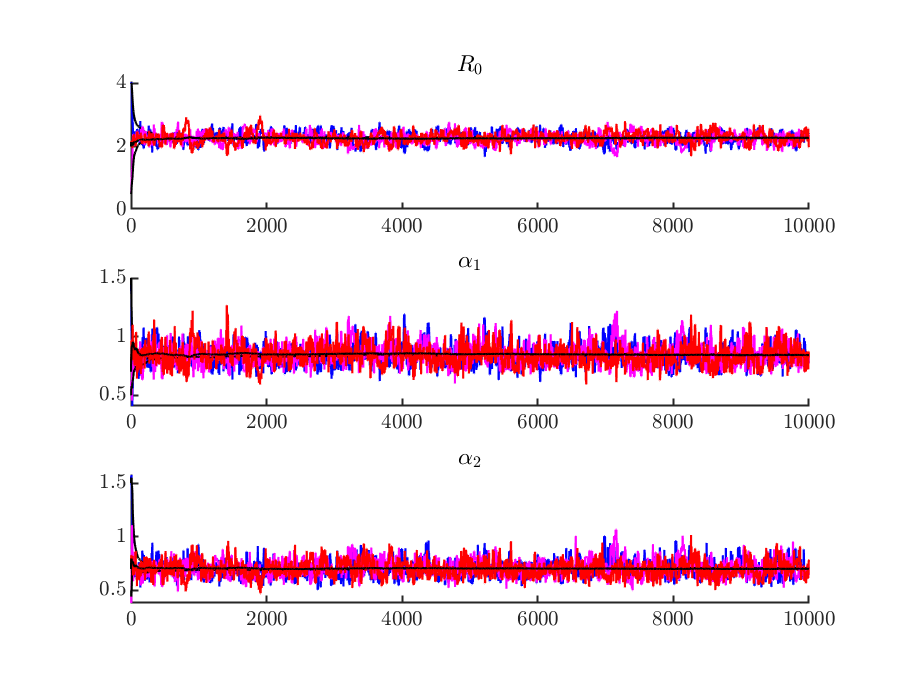
\includegraphics[width=0.8\linewidth]{MHplot0.eps}
	\caption{Superimposed trace plots for the estimations of the parameters from the modified MH algorithm}
	\label{fig:fullrun}
\end{figure}
\begin{figure}[tbh]
	\centering
	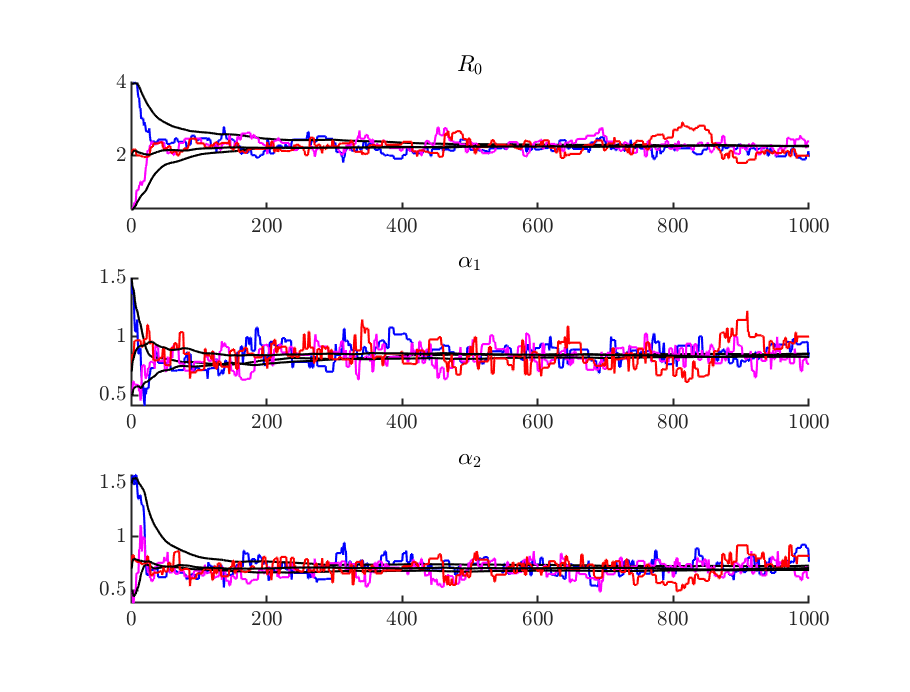
\includegraphics[width=0.8\linewidth]{MHplot1.eps}
	\caption{First 1000 iterations of the MH algorithm. Clearly the burn in has completed after approximately 500 iterations for the three parameters }
	\label{fig:burnin}
\end{figure}


\clearpage

The distributions for $R_0$, $\alpha_1$ and $\alpha_2$ are shown in figure~\ref{fig:density}, where $R_0$ is the reproduction number, $\alpha_1$ and $\alpha_2$ multiply with $R_0$ to get the effective reproduction numbers under $T_1$ and $T_2$ respectively. 
The values stated above correspond to the peaks on these plots, but it is worth acknowledging that there is a reasonable probability that $R_0$ could be between $2$ and $2.6$ and $\alpha_1$ could even be greater than $1$, corresponding to an \textit{increase} in infectivity under $T_1$.



\begin{figure}[tbh]
	\centering
	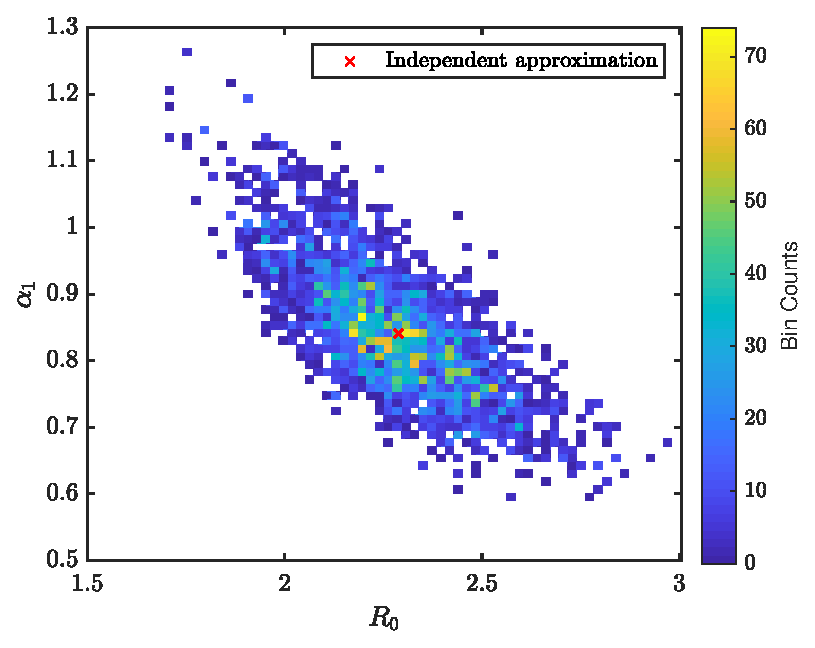
\includegraphics[width=0.45\linewidth]{BinScatter12.eps}
	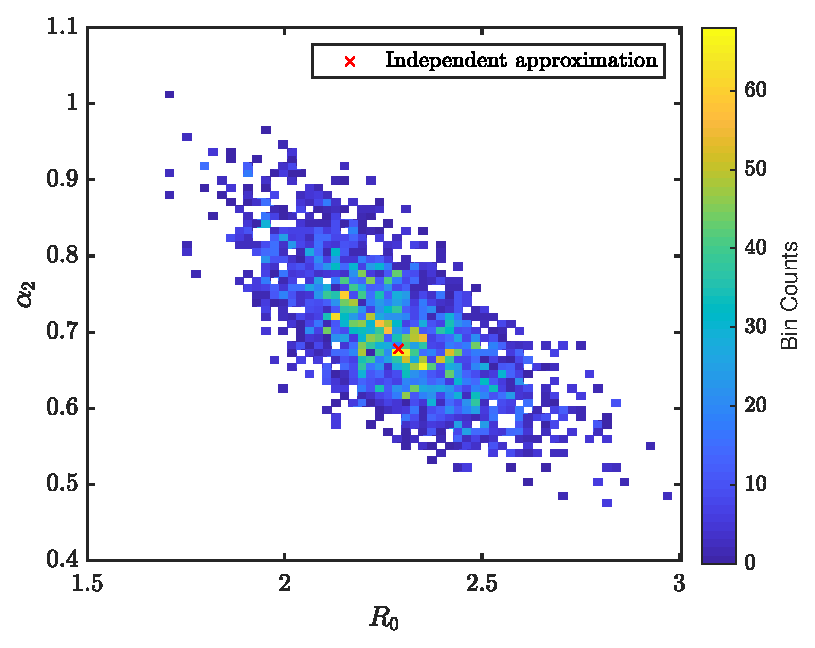
\includegraphics[width=0.45\linewidth]{BinScatter13.eps}
	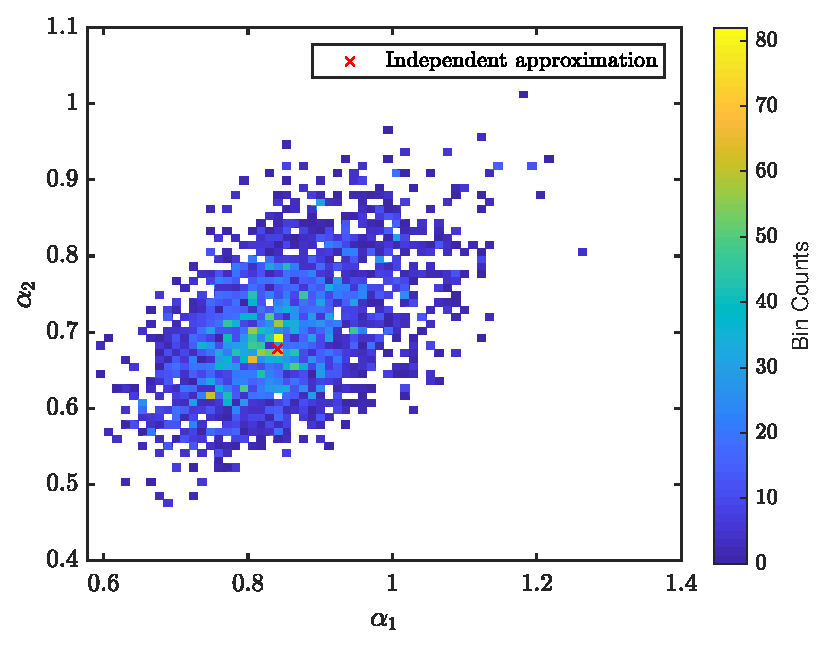
\includegraphics[width=0.45\linewidth]{BinScatter23.eps}
	\caption{Bin scatter plots of the parameters identifying any correlations and their effect on the value. Top-left: $(R_0,\alpha_1)$, Top-right: $(R_0, \alpha_2)$, Bottom: $(\alpha_1,\alpha_2)$}
	\label{fig:binscatter}
\end{figure}


\begin{figure}[tbh]
	\centering
	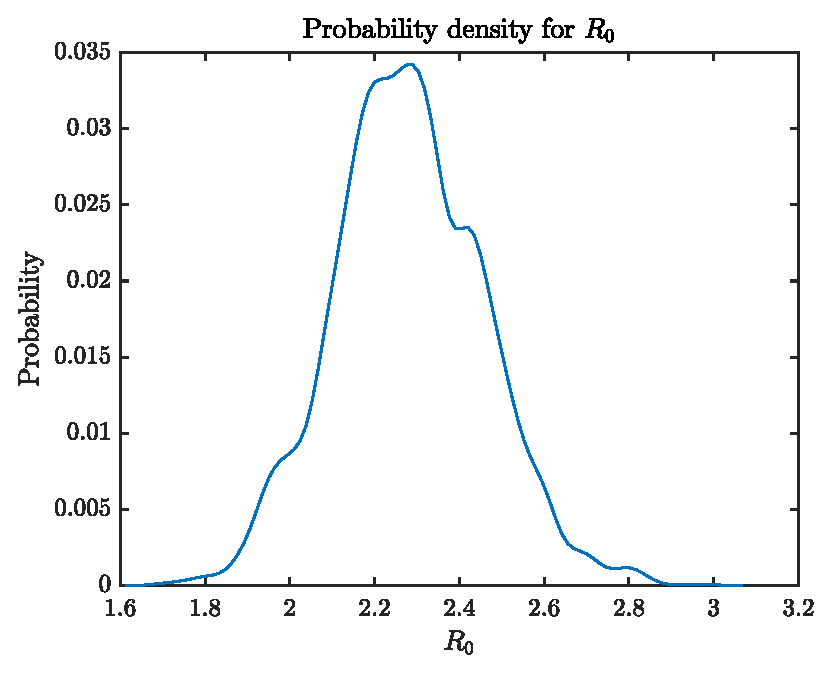
\includegraphics[width=0.45\linewidth]{Probdensity1.eps}
	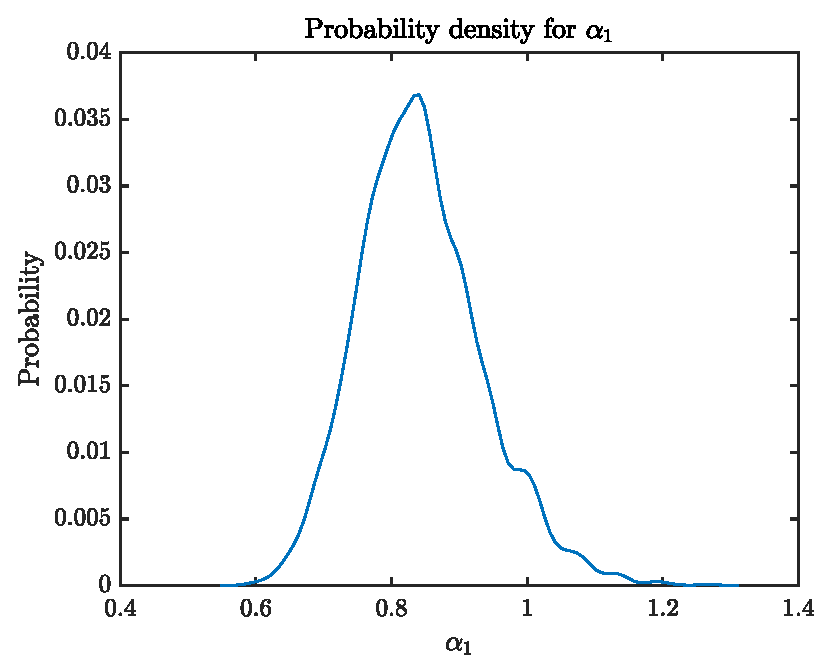
\includegraphics[width=0.45\linewidth]{Probdensity2.eps}
	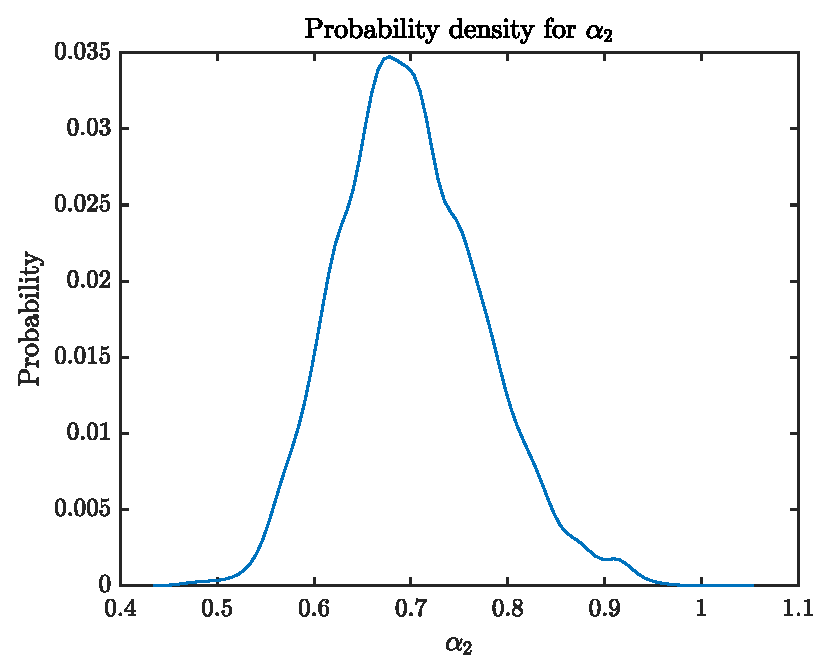
\includegraphics[width=0.45\linewidth]{Probdensity3.eps}
	\caption{Probability density curves for the parameters - the horizontal axis is the parameter while the vertical is the probability}
	\label{fig:density}
\end{figure}




%%%%%%%%%%%%%%%%%%%%%%%%%%%%%%%%%%%%%%%%%%%%%%%%%%%%%%%%%%%%%%%%%%%%%%%%%%%%%%%%%%%%%%%%%
\section{Conclusion}

The effective reproduction numbers, $R_0$ for the control and two treatment types are found to be, respectively, $2.2883$, $1.9242$ and $1.5518$. The two independent treatments appear to have had positive effects on the reproduction number, with treatment 2, $T_2$ appearing to be the most effective. 

The treatments still do not reduce $R_0$ below the threshold of $R_0 =1$, meaning the treatments do not remove the possibility of major outbreaks. For now $T_2$ should still be implemented as it is a significant improvement on taking no action. However, more research should be taken to attempt to find a more effective treatment.


%%%%%%%%%%%%%%%%%%%%%%%%%%%%%%%%%%%%%%%%%%%%%%%%%%%%%%%%%%%%%%%%%%%%%%%%%%%%%%%%%%%%%%%%%%%
\clearpage


\appendix

\printbibliography
\section{Code}
\subsection{Main Script (R0Predict.m)}
\lstinputlisting{R0Predict.m}

\subsection{MetropolisHastingsPassLikelihood.m}
\lstinputlisting{MetropolisHastingsPassLikelihood.m}
\subsection{LogLikelihood.m}
\lstinputlisting{LogLikelihood.m}
\subsection{ProposalConstraints.m}
\lstinputlisting{ProposalConstraints.m}



%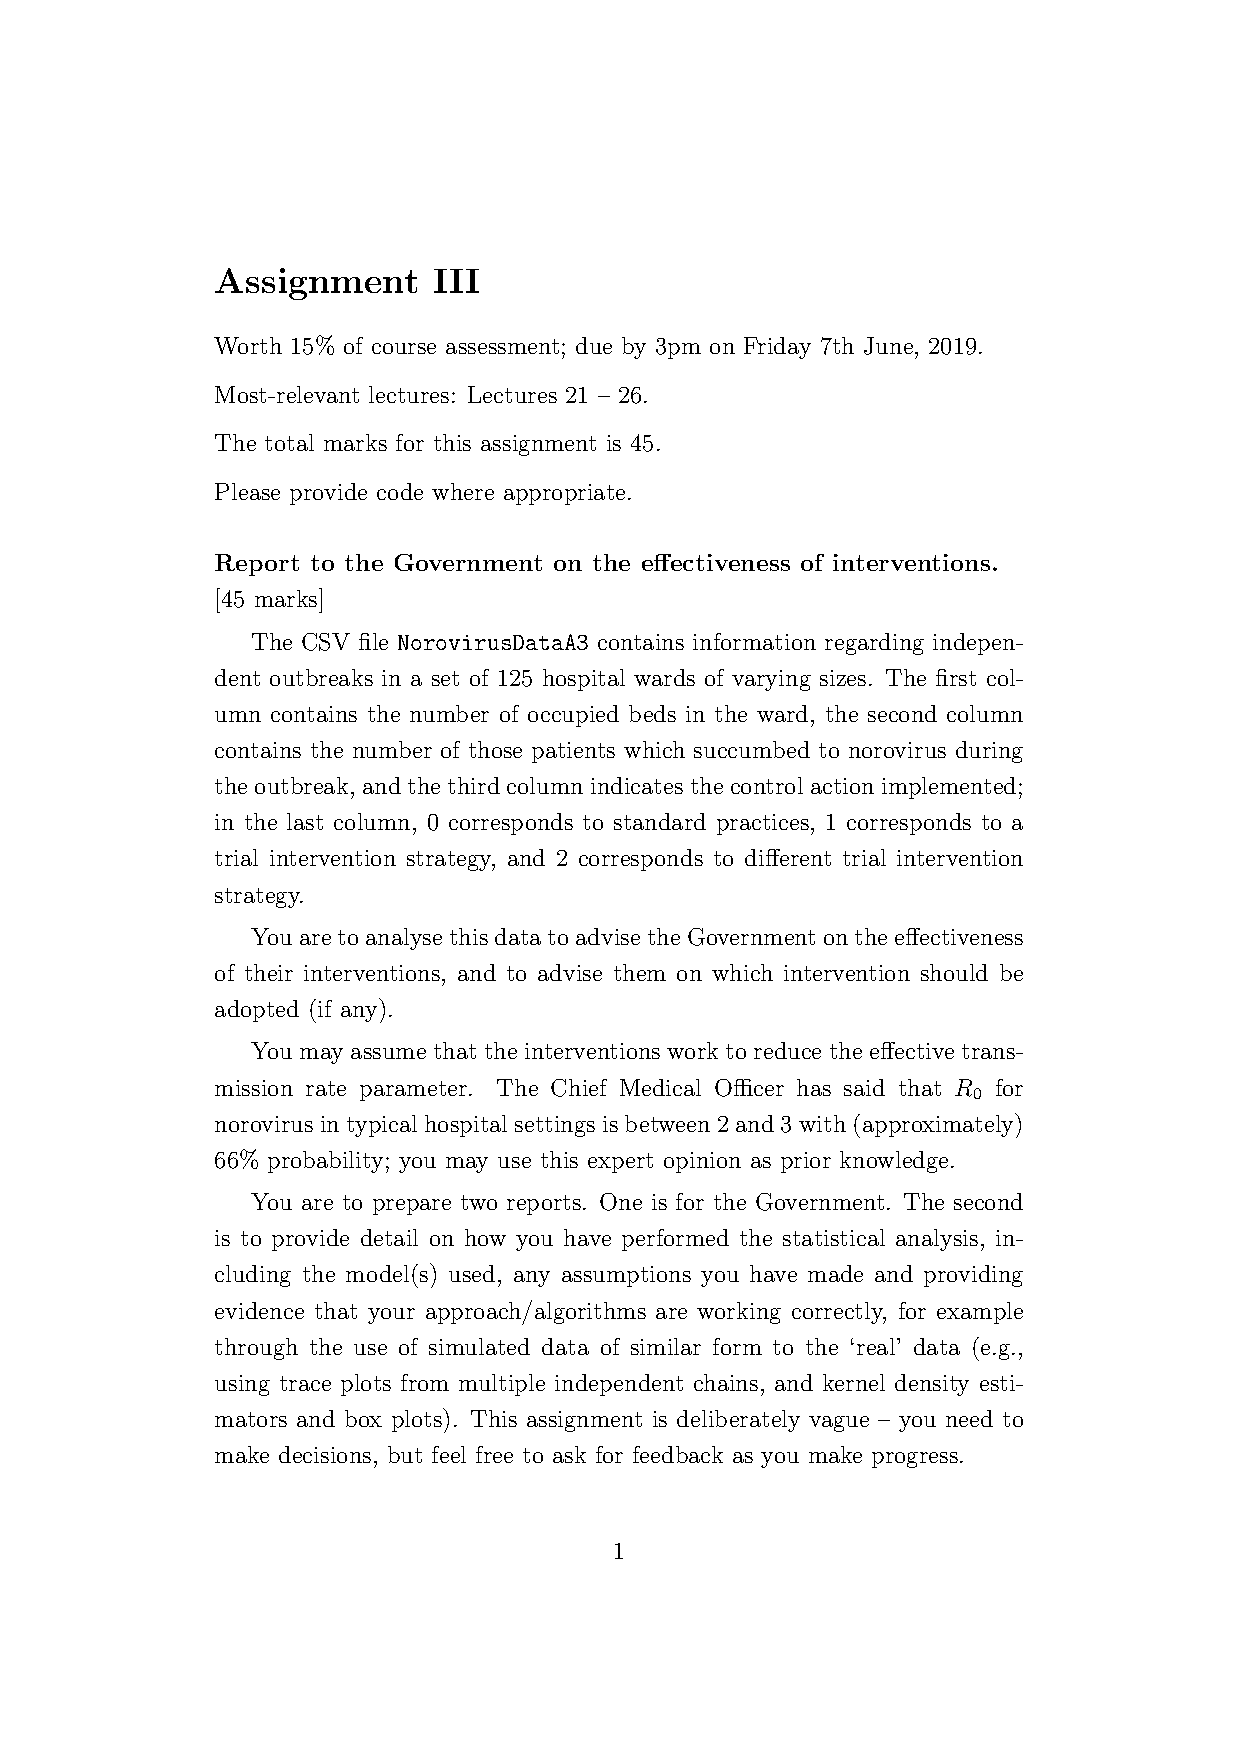
\includepdf[pages=1-]{Honours2019Assignment3}
\end{document}